\section{Group -- Room Air Models}\label{group-room-air-models}

\subsection{Room Air Models}\label{room-air-models}

The group of input objects described in this section is used to account for non-uniform room air temperatures that may occur within the interior air volume of a zone. Room air modeling was added to EnergyPlus starting with Version 1.2. Although there are many types of analyses (comfort, indoor air quality, etc) that might benefit from localized modeling of how room air varies across space, only the \emph{temperature} distribution of room air within the zone is currently addressed in EnergyPlus. This allows surface heat transfer and air system heat balance calculations to be made taking into account natural thermal stratification of air and different types of intentional air distribution designs such as under-floor and side-wall displacement ventilation that purport to extract room air at higher-than-mean temperatures. Note that EnergyPlus does \textbf{not} have completely general methods of modeling room air that are applicable to every conceivable type of airflow that might occur in a zone. Such models (e.g.~RANS-CFD) are too computationally expensive to use with EnergyPlus for the foreseeable future. The models that are available in EnergyPlus offer only limited modeling capabilities for select room airflow configurations. Also note that because the complete mixing model for room air has long been the standard in building energy simulation, there is not currently a consensus on how to best model non-uniform air temperatures in buildings. Therefore, it is up to the user to have a good understanding of when, where, and how to apply the room air models available in EnergyPlus. The rest of this section provides some guidance in the way of examples and further discussion of the models available in EnergyPlus.

EnergyPlus offers the different types of air models listed in the table below along with the input objects associated with the use of that model.

% table 10
{\scriptsize
\begin{longtable}[c]{p{1.5in}p{1.5in}p{1.5in}p{1.5in}}
\caption{Summary of Room Air Models \label{table:summary-of-room-air-models}} \tabularnewline
\toprule
Air Model Key & Air model Algorithm & Applicability & Input Objects Required \tabularnewline
\midrule
\endfirsthead

\caption[]{Summary of Room Air Models} \tabularnewline
\toprule
Air Model Key & Air model Algorithm & Applicability & Input Objects Required \tabularnewline
\midrule
\endhead

Mixing & Well-Mixed & All zones & None, default \tabularnewline
UserDefined & User Defined & All zones & `Room\-Air\-Model\-Type', `Room\-Air:\-Temperature\-Pattern:\-User\-Defined', `Room\-Air:\-Temperature\-Pattern:***' \tabularnewline
One\-Node\-Displacement\-Ventilation & Mundt & displacement ventilation & `Room\-Air\-Model\-Type', `Room\-Air\-Settings:\-One\-Node\-Displacement\-Ventilation', `Room\-Air:Node' \tabularnewline
Three\-Node\-Displacement\-Ventilation & UCSD Displacement Ventilation & displacement ventilation & `Room\-Air\-Model\-Type', `Room\-Air\-Settings:\-Three\-Node\-Displacement\-Ventilation' \tabularnewline
Under\-Floor\-Air\-Distribution\-Interior & UCSD UFAD Interior Model & Interior zones served by a UFAD system & `Room\-Air\-Model\-Type', `Room\-Air\-Settings:\-Under\-Floor\-Air\-Distribution\-Interior' \tabularnewline
Under\-Floor\-Air\-Distribution\-Exterior & UCSD UFAD Exterior Model & Exterior zones served by a UFAD system & `Room\-Air\-Model\-Type', `Room\-Air\-Settings:\-Under\-Floor\-Air\-Distribution\-Exterior' \tabularnewline
Cross\-Ventilation & UCSD Cross Ventilation & cross ventilation & `Room\-Air\-Model\-Type', `Room\-Air\-Settings:\-Cross\-Ventilation' \tabularnewline
\bottomrule
\end{longtable}
}

\subsection{RoomAirModelType}\label{roomairmodeltype}

EnergyPlus uses the Room\-Air\-Model\-Type object to determine which air model is available for use in a given zone during the simulation. If no Room\-Air\-Model\-Type object is specified (for each zone or the whole building), then EnergyPlus will run with the conventional, completely mixing air model (for each zone or the whole building). Include a Room\-Air\-Model\-Type for each zone that the user wants modeled using a more detailed method. Currently only a single Room\-Air\-Model\-Type object can be specified for each zone; you cannot switch between models during a simulation. However, the UCSD Displacement, Cross Ventilation and UFAD models switch from displacement to mixing ventilation when the operating conditions do not give rise to unmixed flow. The following parameters are fields required by the Room\-Air\-Model\-Type object.

\subsubsection{Inputs}\label{inputs-041}

\paragraph{Field: Name}\label{field-name-040}

This alpha field is the air model name selected by user. It is used as an identifier

\paragraph{Field: Zone Name}\label{field-zone-name-011}

This alpha field indicates the unique name of a Zone object defined elsewhere in the input file. The type of room air model selected will be applied to this zone.

\paragraph{Field: Room-Air Modeling Type}\label{field-room-air-modeling-type}

This alpha field indicates the room-air model used for the specified zone. Currently, there are three options for different air models. Entering the keyword `Mixing' specifies the conventional complete-mixing air model. Note that Mixing is the default and no Room\-Air\-Model\-Type object would be needed to use the complete-mixing model. Entering the keyword `UserDefined `specifies the User Defined Room Air Temperature Patterns. Entering the keyword `OneNodeDisplacementVentilation `specifies the Mundt one node displacement ventilation air model for displacement ventilation. Entering the keyword `ThreeNodeDisplacementVentilation` specifies the three-node displacement ventilation model developed by the University of California, San Diego (UCSD DV). Entering the keyword `CrossVentilation' specifies the two-zone cross ventilation model developed by the University of California, San Diego (UCSD CV). Entering the keyword `UnderFloorAirDistributionInterior` specifies the two-node interior zone under floor air distribution model developed by the University of California, San Diego (UCSD UFI). Entering the keyword `UnderFloorAirDistributionExterior` specifies the two-node exterior zone under floor air distribution model developed by the University of California, San Diego (UCSD UFE).

\paragraph{Field: Air Temperature Coupling Strategy}\label{field-air-temperature-coupling-strategy}

This alpha field indicates how air temperatures predicted by the air models are used by the surface heat balance calculation. Two different coupling schemes are available: Direct (also known as \emph{T-couple}) or Indirect (\emph{DT-couple}). In general, indirect coupling is more suited to situations where room air is well controlled and/or the room air model is less robust. Direct coupling is more suited for floating zone air temperatures and/or accurate room air models.

The Mundt model can use either coupling scheme; the UCSD DV, UCSD CV, UCSD UFI, and UCSD UFE models ignore this field and use direct coupling.

Input either \emph{Direct} or \emph{Indirect}

An example idf entry follows

\begin{lstlisting}
RoomAirModelType,
  MOD1,                             !- Room-Air Model Name
  ZONE ONE,                         !- Zone Name
  ThreeNodeDisplacementVentilation, !- Room-Air Modeling Type
  Direct;                           !- Air Temperature Coupling Strategy
\end{lstlisting}

\subsection{RoomAir:TemperaturePattern:UserDefined}\label{roomairtemperaturepatternuserdefined}

This object is used to explicitly define temperature patterns that are to be applied to the mean air temperature within a thermal zone. This Room Air modeling option is made available for a number of reasons. It allows modeling the consequences of air temperature variations during the design phase when little information is available about the specifics of the air distribution system or positioning of various loads. This option can be used to evaluate the energy implications of different design targets for the temperature patterns. It also provides a method of modeling the annual energy use implications for air temperature distributions determined using separate analyses or measurements. For example, this option could be used to understand the annual energy implications of an air distribution system that has been previously analyzed using Computational Fluid Dynamics.

This approach differs from the other Room Air modeling in that the static temperature pattern is not really \emph{modeled} so that it will respond to conditions that develop during the simulation. More sophisticated dynamic Room Air models will adjust the temperature pattern based on various factors, such as air system flow rate, floor temperature, or rates of internal heat gains. The user-defined temperature distribution patterns are fixed at the beginning and EnergyPlus simply provides results that include the implications of those patterns. This user-defined distribution option may also be useful for checking dynamic Room Air models by using ``bounding'' analysis.

Note that using this object carries a certain degree of responsibility. It would be very easy to define a pattern that is non-physical and will lead to erroneous results. The user-defined temperature distributions should (probably) be balanced about the mean so that basic conservation of energy laws are not violated.

\subsubsection{Inputs}\label{inputs-1-038}

\paragraph{Field: Name}\label{field-name-1-037}

This field provides a unique name for this object.

\paragraph{Field: Zone Name}\label{field-zone-name-1-008}

This field provides the unique name of a zone described elsewhere in the file.

\paragraph{Field: Availability Schedule Name}\label{field-availability-schedule-name-015}

This field provides the name of a schedule that will determine if this model is available. When not available the room air is modeled as completely mixed. When it is available, then a user-defined temperature distribution will be applied. This schedule should be set to ``1.0'' when model is available and ``0.0'' when the model is not to be used. If this field is blank, the schedule has values of 1 for all time periods.

\paragraph{Field: Pattern Control Schedule Name}\label{field-pattern-control-schedule-name}

This field provides the name of schedule that will be used to control which user-defined RoomAir temperature pattern will be applied at any given time. This schedule needs to have integer values that are closely coordinated with those defined as the second field in one of the RoomAir:TemperaturePattern:* objects described below. These schedule values provide the link to the actual patterns to be used throughout the day. This allows controlling which user-defined pattern is used at different times during the simulation. For example, one could use one pattern when the air system is scheduled to be on, and a different pattern when the air system is schedule to be off. Or if the user has knowledge of how the air temperature pattern changes over the course of day in response to changing thermal loads, then this schedule can be used to control when individual patterns are used. For example, a control schedule could use a pattern designated as number 100 from 18:00 to 6:00, pattern number 200 from 6:00 to 12:00, and pattern number 300 from 12:00 to 18:00.

An example of this object is

\begin{lstlisting}
RoomAir:TemperaturePattern:UserDefined,
  Ground Floor South Air Temp Controls,  ! Name
  ZN2_S_1,                              ! Zone Name
  Always_on,                            ! Availability Schedule Name
  Roomair Pattern 1;                    ! Pattern Control Schedule Name
\end{lstlisting}

\subsection{RoomAir:TemperaturePattern:ConstantGradient}\label{roomairtemperaturepatternconstantgradient}

This object is used to model room air with a fixed temperature gradient in the vertical direction. This fixed-slope method is about the simplest distribution pattern.

In addition to the vertical temperature gradient, there are three other parameters included in the pattern that are important. The first two might affect how the air system conditioning the room is operated. The first describes the temperature difference between the mean air temperature and the point where the sensor of a drybulb thermostat is situated. The second describes the temperature difference between the mean and the point where system air is being extracted from the zone. This is considered important because the changes in temperature difference between supply and return can affect how an air system is controlled to meet the loads. The third parameter can affect the zone air heat balance by altering the temperature of the air leaving the zone through exhaust fans.

One example of a source of input data for the vertical temperature gradient is ANSI/ASHRAE Standard 55-2004 Thermal Environmental Conditions for Human Occupancy. Table 5.2.4.3 in this Standard specifies an allowable vertical temperature difference between head level and ankle level of 3ºC (5ºF). If we assume a head to ankle length scale of 1.5 m (5 ft), this leads to a temperature gradient of 3ºC/1.5m, or 2.0 ºC/m.

\subsubsection{Inputs}\label{inputs-2-035}

\paragraph{Field: Name}\label{field-name-2-033}

This field provides a unique name for this object.

\paragraph{Field: Control Integer for Pattern Control Schedule Name}\label{field-control-integer-for-pattern-control-schedule-name}

This field should contain an integer value that is unique among all other RoomAir:TemperaturePattern:* objects. The value used here needs to be in the Pattern Control Schedule for those times when this pattern is to be used for the Room Air Temperature Distribution.

\paragraph{Field: Thermostat Offset}\label{field-thermostat-offset}

This field specifies the temperature difference between where the thermostat is situated and the mean air temperature.

\paragraph{Field: Return Air Offset}\label{field-return-air-offset}

This field specifies the temperature difference between the air leaving the zone and returning to the air system and the mean air temperature.

\paragraph{Field: Exhaust Air Offset}\label{field-exhaust-air-offset}

This field specifies the temperature difference between the air leaving the zone and being exhausted out of the building and the mean air temperature.

\paragraph{Field: Temperature Gradient}\label{field-temperature-gradient}

This field specifies the gradient, or slope, of temperature changes in the vertical direction in ºK/m.

An example of this object is:

\begin{lstlisting}
RoomAir:TemperaturePattern:ConstantGradient,
  half C per Meter,     ! Name
  10005,                ! Control Integer for Pattern Control Schedule Name
  0.0,                  ! Thermostat Offset (Temp at thermostat- Mean Air Temp) [C]
  1.0,                  ! Return Air Offset (Tleaving - Mean Air Temp )  [C]
  1.0,                  ! Exhaust Air Offset (Texhaust - Mean Air Temp)  [C]
  0.5;                  ! Temperature Gradient [K/m]
\end{lstlisting}

\subsection{RoomAir:TemperaturePattern:TwoGradient}\label{roomairtemperaturepatterntwogradient}

This object provides various controls over the value of the gradient used for determining the pattern of room air temperatures. It is similar to previous object \hyperref[roomairtemperaturepatternconstantgradient]{RoomAir:TemperaturePattern:ConstantGradient} object but simplifies the potentially arduous task of preparing and scheduling a large number of those objects. With this object, two different gradients are entered and user is given several options for controlling how the program will interpolate between the two bounds. The user inputs the height of the location of thermostat, return air, and exhaust air in meters rather than the temperature offset.

\subsubsection{Inputs}\label{inputs-3-031}

\paragraph{Field: Name}\label{field-name-3-027}

This field provides a unique name for this object.

\paragraph{Field: Control Integer for Pattern Control Schedule Name}\label{field-control-integer-for-pattern-control-schedule-name-1}

This field should contain an integer value that is unique among all other RoomAir:TemperaturePattern:* objects. The value used here needs to be in the Pattern Control Schedule for those times when this pattern is to be used for the Room Air Temperature Distribution.

\paragraph{Field: Thermostat Height}\label{field-thermostat-height}

This field specifies the distance above the floor where the thermostat is situated. This height is used by the model to determine the thermostat temperature relative to the mean air temperature by applying the gradient.

\paragraph{Field: Return Air Height}\label{field-return-air-height}

This field specifies the distance above the floor where the air leaves the zone and returns to the air system. and the mean air temperature. This height is used by the model to determine the return air temperature relative to the mean air temperature by applying the gradient.

\paragraph{Field: Exhaust Air Height}\label{field-exhaust-air-height}

This field specifies the distance above the floor where the air leaves the zone and enters and exhaust device such as an exhaust fan. This height is used by the model to determine the exhaust air temperature relative to the mean air temperature by applying the gradient.

\paragraph{Field: Temperature Gradient Lower Bound}\label{field-temperature-gradient-lower-bound}

This field specifies the gradient, or slope, of temperature changes in the vertical direction in ºC/m.

\paragraph{Field: Temperature Gradient Upper Bound}\label{field-temperature-gradient-upper-bound}

This field specifies the gradient, or slope, of temperature changes in the vertical direction in ºC/m.

\paragraph{Field: Gradient Interpolation Mode}\label{field-gradient-interpolation-mode}

This field specifics how the program will vary between the two gradients. Select one of the following keywords to choose the simulation data used to scale: `Outdoor Environment Drybulb Temperature', `Zone Drybulb Temperature', `Delta Outdoor and Zone Temperature', `Sensible Cooling Load', and `Sensible Heating Load'. These are explained in detail below. All of these options have several things in common. They are essentially hard-coded. There is no support for a general method. The interpolation scheme is based on some variable that might reasonably be expected to correlate with gradient changes. This variable's current value is used to continually adjust the value of the vertical gradient for room air temperature.

\textbf{OutdoorDryBulbTemperature:} This key directs the program to interpolate between upper and lower values of the vertical gradient based on the outdoor air temperature. If the outdoor temperature exceeds the upper limit set in the next field, then the gradient entered in the `Temperature Gradient Upper Bound' field is used. Similarly if the outdoor air temperature is below the value set in the `Lower Temperature' field, then the gradient entered in the `Temperature Gradient Lower Bound' is used. For outdoor temperatures that lie between the upper and lower bounds, the gradient is determined by linear interpolation between the two.

\textbf{ZoneDryBulbTemperature}: This key directs the program to interpolate between upper and lower values of the vertical gradient based on the mean zone air temperature. If the mean zone air temperature exceeds the upper limit set in the next field, then the gradient entered in the `Temperature Gradient Upper Bound' field is used. Similarly if the mean zone air temperature is below the value set in the `Lower Temperature' field, then the gradient entered in the `Temperature Gradient Lower Bound' is used. For mean zone air temperatures that lie between the upper and lower bounds, the gradient is determined by linear interpolation between the two.

\textbf{ZoneAndOutdoorTemperatureDifference}: This key directs the program to interpolate between upper and lower values of the vertical gradient based on the difference between the outdoor environment and the mean zone air temperature. If the temperature difference exceeds the upper limit set in the next field, then the gradient entered in the `Temperature Gradient Upper Bound' field is used. Similarly if the temperature difference is below the value set in the `Lower Temperature' field, then the gradient entered in the `Temperature Gradient Lower Bound' is used. For temperature differences that lie between the upper and lower bounds, the gradient is determined by linear interpolation between the two.

\textbf{SensibleCoolingLoad}: This key directs the program to interpolate between upper and lower values of the vertical gradient based on the sensible cooling load. If the cooling load exceeds the upper limit set in the next field, then the gradient entered in the `Temperature Gradient Upper Bound' field is used. Similarly if the cooling load is below the value set in the `Lower Temperature' field, then the gradient entered in the `Temperature Gradient Lower Bound' is used. For cooling loads that lie between the upper and lower bounds, the gradient is determined by linear interpolation between the two.

\textbf{SensibleHeatingLoad}: This key directs the program to interpolate between upper and lower values of the vertical gradient based on the sensible heating load. If the heating load exceeds the upper limit set in the next field, then the gradient entered in the `Temperature Gradient Upper Bound' field is used. Similarly if the heating load is below the value set in the `Lower Temperature' field, then the gradient entered in the `Temperature Gradient Lower Bound' is used. For heating loads that lie between the upper and lower bounds, the gradient is determined by linear interpolation between the two.

\paragraph{Field: Upper Temperature Bound}\label{field-upper-temperature-bound}

This field is used to enter the upper bound on temperature values in Celsius. It is required for the interpolation modes based on temperature.

\paragraph{Field: Lower Temperature Bound}\label{field-lower-temperature-bound}

This field is used to enter the lower bound on temperature values in Celsius. It is required for the interpolation modes based on temperature.

\paragraph{Field: Upper Heat Rate Bound}\label{field-upper-heat-rate-bound}

This field is used to enter the upper bound on heat rate values. It is required for the interpolation modes based on load. Both heating and cooling loads are entered as positive numbers (in watts).

\paragraph{Field: Lower Heat Rate Bound}\label{field-lower-heat-rate-bound}

This field is used to enter the lower bound on heat rate values. It is required for the interpolation modes based on load. Both heating and cooling loads are entered as positive numbers (in watts).

An example of this object follows. This pattern will apply no gradient (effectively the mixing model) if zone air temperatures are 22.5 C or lower. It will apply a gradient of 1 K/m if zone temperatures are 26.0 C or higher. For zone air temperatures between 22.5 and 26.0 it will determine the gradient by linear interpolation and use a gradient between 0.0 and 1.0 K/m depending on where the zone air temperature is in the range.

\begin{lstlisting}
RoomAir:TemperaturePattern:TwoGradient,
  Mixed to one C per M by Zone DB, ! Name
  2002,                   ! Control Integer for Pattern Control Schedule
  1.1,                    ! Thermostat Height meters
  4.5,                    ! Return Air Height
  3.5,                    ! Exhaust Air Height
  0.0,                    ! Temperature Gradient Lower Bound K/m
  1.0,                    ! Temperature Gradient Upper  Bound K/m
  ZoneDrybulbTemperature, ! Gradient Interpolation Mode
  26.0,                   ! Upper Temperature [C]
  22.5,                   ! Lower Temperature [C]
  ,                       ! Upper Heat Rate [W]
  ;                       ! Lower Heat Rate [W]
\end{lstlisting}

\subsubsection{Outputs}\label{roomairtemperaturepatterntwogradient-outputs}

The user-defined air temperature pattern that interpolates between two gradients produces the following output variable.

\begin{lstlisting}
HVAC,Average,Room Air Zone Vertical Temperature Gradient [K/m]
\end{lstlisting}

\paragraph{Room Air Zone Vertical Temperature Gradient {[}K/m{]}}\label{room-air-zone-vertical-temperature-gradient-km}

This output variable is the result of the interpolation performed by the user-defined roomair model using RoomAir:TemperaturePattern:TwoGradient. This is the temperature gradient in the vertical direction. The units are degrees Kelvin per meter.

\subsection{RoomAir:TemperaturePattern:NondimensionalHeight}\label{roomairtemperaturepatternnondimensionalheight}

This object defines a distribution pattern for air temperatures relative to the current mean air temperature as a function of height. The height, referred to as Zeta, is non-dimensional by normalizing with the zone ceiling height. (The actual zone ceiling height can be explicitly entered in the `Zone' object but if not it is calculated by EnergyPlus from the surfaces attached to the zone.) The temperature differences are not non-dimensional and remain in units of degrees Celsius.

An example of a vertical temperature pattern is shown in the figure below. The pattern itself is treated as a piecewise, linear model of air temperature as a function of height. This Zeta-DeltaTai curve, or lookup table, is then mapped to surfaces defined elsewhere in the file. The centroid of each surface and zone ceiling height are used to automatically assign Zeta values within the program. The zone named in the referencing \hyperref[roomairtemperaturepatternuserdefined]{RoomAir:TemperaturePattern:UserDefined} object is used to determine which surfaces will be associated with the pattern when it is applied. A single pattern object can be reused for multiple zones and times.

In addition to the vertical temperature pattern there are three other parameters included in the pattern that are important. The first two might affect how the air system conditioning the room is operated. The first describes the temperature difference between the mean air temperature and the point where the sensor of a drybulb thermostat is situated. The second describes the temperature difference between the mean and the point where system air is being extracted from the zone. This is considered important because the changes in temperature difference between supply and return can affect how an air system is controlled to meet the loads. The third parameter can affect the zone air heat balance by altering the temperature of the air leaving the zone through exhaust fans.

\begin{figure}[hbtp] % fig 44
\centering
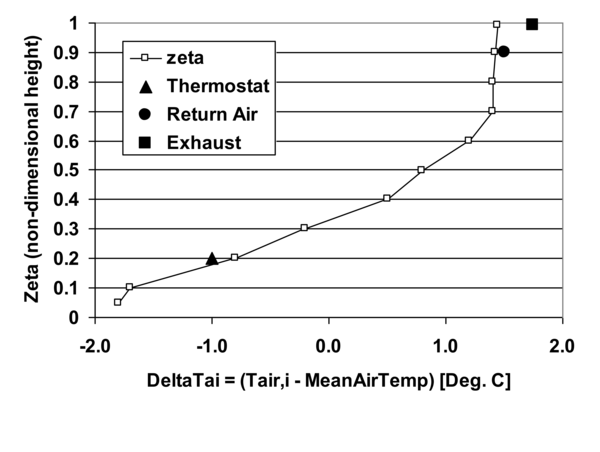
\includegraphics[width=0.9\textwidth, height=0.9\textheight, keepaspectratio=true]{media/image079.png}
\caption{Example of a Vertical Air Temperature Pattern \protect \label{fig:example-of-a-vertical-air-temperature-pattern}}
\end{figure}

\subsubsection{Inputs}\label{inputs-4-028}

\paragraph{Field: Name}\label{field-name-4-024}

This field provides a unique name for this object.

\paragraph{Field: Control Integer for Pattern Control Schedule Name}\label{field-control-integer-for-pattern-control-schedule-name-2}

This field should contain an integer value that is unique among all other RoomAir Temperature Pattern objects. The value used here needs to be in the Pattern Control Schedule for those times when this pattern is to be used for the Room Air Temperature Distribution.

\paragraph{Field: Thermostat Offset}\label{field-thermostat-offset-1}

This field specifies the temperature difference between where the thermostat is situated and the mean air temperature.

\paragraph{Field: Return Air Offset}\label{field-return-air-offset-1}

This field specifies the temperature difference between the air leaving the zone and returning to the air system and the mean air temperature.

\paragraph{Field: Exhaust Air Offset}\label{field-exhaust-air-offset-1}

This field specifies the temperature difference between the air leaving the zone and being exhausted out of the building and the mean air temperature.

\paragraph{Field Set Zeta and Temperature Difference}\label{field-set-zeta-and-temperature-difference}

The remaining fields contain pairs of values that define a lookup table for the temperature pattern in the vertical direction. The first value is Zeta and the second value is DeltaTai.

\paragraph{Field: Pair \textless{}\#\textgreater{} Zeta non-dimensional Height}\label{field-pair-zeta-non-dimensional-height}

Zeta is the normalized height and should be a fractional value from 0.0 to 1.0. A value of 0.0 corresponds to the floor and a value of 1.0 corresponds to the ceiling. The Zeta values need to be in increasing value.

\paragraph{Field: Pair \textless{}\#\textgreater{} Delta Adjacent Air Temperature}\label{field-pair-delta-adjacent-air-temperature}

DeltaT\(_{ai}\) is the temperature difference between the air temperature at the associated Zeta (T\(_{ai}\)) and the mean air temperature and is given in degrees Celsius.

This object is extensible, so additional pairs of these last two fields of this type can be added to the end of this object. An example of this object corresponding to the figure above is:

\begin{lstlisting}
RoomAir:TemperaturePattern:NondimensionalHeight,
  Rough UFAD Approx,    ! Name
  3001,                 ! Control Integer for Pattern Control Schedule
                        ! note reference this entry in Schedule
  -1.0 ,                ! Thermostat Offset
  1.5 ,                 ! Return Air Offset (Tleaving - Mean Air Temp ) deg C
  1.75,                 ! Exhaust Air Offset (Texhaust - Mean Air Temp) deg C
  0.05,  -1.8,          ! pair 1 (Zeta , DeltaTai)
  0.1,   -1.7,          ! pair 2 (Zeta , DeltaTai)
  0.2,   -0.8,          ! pair 3 (Zeta , DeltaTai)
  0.3,   -0.2,          ! pair 4 (Zeta , DeltaTai)
  0.4,    0.5,          ! pair 5 (Zeta , DeltaTai)
  0.5,    0.8,          ! pair 6 (Zeta , DeltaTai)
  0.6,    1.2,          ! pair 7 (Zeta , DeltaTai)
  0.7,    1.4,          ! pair 8 (Zeta , DeltaTai)
  0.8,    1.4,          ! pair 9 (Zeta , DeltaTai)
  0.9,   1.42,          ! pair 10 (Zeta , DeltaTai)
  0.95,  1.44;          ! pair 11 (Zeta , DeltaTai)
\end{lstlisting}

\subsection{RoomAir:TemperaturePattern:SurfaceMapping}\label{roomairtemperaturepatternsurfacemapping}

This object defines a distribution pattern for the air temperatures adjacent to individual surfaces. This object uses the specific names of individual surfaces defined elsewhere in the model. This pattern allows controlling the adjacent air temperature on a surface-by-surface basis rather than by height. This allows modeling different adjacent air temperatures on the opposite sides of the zone.

In addition to the surface mappings there are three other parameters included in the pattern that are important. The first two might affect how the air system conditioning the room is operated. The first describes the temperature difference between the mean air temperature and the point where the sensor of a drybulb thermostat is situated. The second describes the temperature difference between the mean and the point where system air is being extracted from the zone. This is considered important because the changes in temperature difference between supply and return can affect how an air system is controlled to meet the loads. The third parameter can affect the zone air heat balance by altering the temperature of the air leaving the zone through exhaust fans.

\subsubsection{Inputs}\label{inputs-5-025}

\paragraph{Field: Name}\label{field-name-5-020}

This field provides a unique name for this object.

\paragraph{Field: Control Integer for Pattern Control Schedule Name}\label{field-control-integer-for-pattern-control-schedule-name-3}

This field should contain an integer value that is unique among all other RoomAir Temperature Pattern objects. The value used here needs to be in the Pattern Control Schedule for those times when this pattern is to be used for the RoomAir Temperature Distribution.

\paragraph{Field: Thermostat Offset}\label{field-thermostat-offset-2}

This field specifies the temperature difference between where the thermostat is situated and the mean air temperature.

\paragraph{Field: Return Air Offset}\label{field-return-air-offset-2}

This field specifies the temperature difference between the air leaving the zone and returning to the air system and the mean air temperature.

\paragraph{Field: Exhaust Air Offset}\label{field-exhaust-air-offset-2}

This field specifies the temperature difference between the air leaving the zone and being exhausted out of the building and the mean air temperature.

\paragraph{Field Set: Surface Name, Temperature Difference}\label{field-set-surface-name-temperature-difference}

\paragraph{Fields (6 and on): Pairs of Surface Names and Temperature Differences}\label{fields-6-and-on-pairs-of-surface-names-and-temperature-differences}

The remaining fields contain pairs that define a lookup table for the temperature pattern on a surface-by-surface basis.

\paragraph{Field: Surface Name Pair \textless{}\#\textgreater{}}\label{field-surface-name-pair}

The name of a surface defined elsewhere in the input file.

\paragraph{Field: Delta Adjacent Air Temperature Pair \textless{}\#\textgreater{}}\label{field-delta-adjacent-air-temperature-pair}

DeltaT\(_{ai}\) is the temperature difference between the air temperature adjacent to the associated surface (T\(_{ai}\)) and the mean air temperature and is given in degrees Celsius.

This object is extensible, so additional pairs of fields of these types can be added to the end of this object.  An example of this object, which might be used to elevate temperatures near west windows in the afternoon, is:

\begin{lstlisting}

RoomAir:TemperaturePattern:SurfaceMapping,
    GroundFloor SW Corner Hot Near West Wall, ! Name
    4001, ! Control Integer for Pattern Control Schedule Name
    0.0, ! Thermostat Offset(Temp at thermostat- Mean Air Temp)
    0.0, ! Return Air Offset  deg C
    0.0, ! Exhaust Air Offset
    ZN1_SW_1:W_ExtWall:1 ,  0.8,  ! pair 1 (Surface Name , DeltaTai)
    ZN1_SW_1:W_ExtWall:2 ,  0.9,  ! pair 2 (Surface Name , DeltaTai)
    ZN1_SW_1:W_ExtWall:3 ,  1.0,  ! pair 3 (Surface Name , DeltaTai)
    ZN1_SW_1:W_ExtWall:4,   1.1,  ! pair 4 (Surface Name , DeltaTai)
    ZN1_SW_1:W_ExtWall:5,   1.3,  ! pair 5 (Surface Name , DeltaTai)
    ZN1_SW_1:W_ExtWall:6,   1.5,  ! pair 6 (Surface Name , DeltaTai)
    ZN1_SW_1:W_ExtWall:7,   1.7,  ! pair 7 (Surface Name , DeltaTai)
    ZN1_SW_1:W_ExtWall:8,   2.1,  ! pair 8 (Surface Name , DeltaTai)
    ZN1_SW_1:W_ExtWall:9,   2.4 ; ! pair 8 (Surface Name , DeltaTai)
\end{lstlisting}

\subsection{RoomAir:Node}\label{roomairnode}

The RoomAir:Node object is used to define air nodes for a nodal air model. The number of air node objects that need to be specified depends on the nodal air model selected. (However, currently only the Mundt model uses this object). In order to use the Mundt model, the user must specify six or more RoomAir:Node objects of different types for each zone. The exact number of RoomAir:Node in the model will vary based on the resolution of walls. If walls (heat transfer surfaces) are split into separate segments in the vertical direction, then more air nodes of type `MundtRoom' will be useful. At a minimum, for the Mundt model RoomAir Nodes of the following type are required: `Inlet, `Floor, `Control, `Ceiling, `MundtRoom, and `Return.'

\subsubsection{Inputs}\label{inputs-6-022}

\paragraph{Field: Name}\label{field-name-6-018}

This alpha field is a name for the air node. It should be unique and is used as an identifier

\paragraph{Field: Node Type}\label{field-node-type}

This alpha field indicates the type of this air node. The following explains options available for use with the Mundt nodal air model.

\textbf{Inlet} is specified for the air node located where the system air enters the zone.

\textbf{Floor} is specified for the air node located near the floor.

\textbf{Control} is specified for the air node located near the thermostat.

\textbf{Ceiling} is specified for the air node located near the ceiling.

\textbf{MundtRoom} is specified for the air node located adjacent to the wall(s).

\textbf{Return} is specified for the air node located where the system air leaves the zone.

\paragraph{Field: Zone Name}\label{field-zone-name-2-006}

This field indicates the name of the zone (Ref: Zone) that this air node belongs to. This should be the unique name of a zone object defined elsewhere in the input file.

\paragraph{Field: Height of Nodal Control Volume Center}\label{field-height-of-nodal-control-volume-center}

This numeric field indicates the height of the air node center. Air models such as the Mundt model compute the air temperature as a function of height and the value entered here will be used to determine a result for this node. The value should be specified in meters and relative to the floor of the zone.

\paragraph{Field: Surface \textless{}\#\textgreater{} Name}\label{field-surface-name-004}

These remaining alpha fields indicate the names of the surfaces (Ref: Surface) that are interacting convectively with this air node. This field is optional and related to the previous field. Currently, at most 20 surfaces are allowed to interact with a single air node. Only those nodes that interact with the inside faces of surfaces need to specify surface names. Each surface should couple to no more than 1 node.

An IDF example:

\begin{lstlisting}

RoomAir:Node,
      WESTZN:FLOORAIR,    !- Node Name
      Floor,      !- Node Type
      WEST ZONE,  !- Name of Zone to Which the Air Node Belongs
      0.1,        !- Height of Nodal Control Volume Center {m}
      WESTZN:FLOOR:LEFF,  !- surface name
      WESTZN:FLOOR:RIGHT; !- surface name
\end{lstlisting}

\subsection{RoomAirSettings:OneNodeDisplacementVentilation}\label{roomairsettingsonenodedisplacementventilation}

The RoomAirSettings:OneNodeDisplacementVentilation object is used to specify additional input parameters required by the Mundt model that are not available in other input objects in EnergyPlus. A single object will be used for the zone.

\subsubsection{Inputs}\label{inputs-7-022}

\paragraph{Field: Zone Name}\label{field-zone-name-3-005}

This alpha field indicates the name of the zone (Ref: Zone) for the required input parameters as specified in the following fields.

\paragraph{Field: Fraction of Convective Internal Loads Added to Floor Air}\label{field-fraction-of-convective-internal-loads-added-to-floor-air}

This numeric field indicates what fraction of the convective part of the internal gains is added to the air near the floor in the zone specified.

\paragraph{Field: Fraction of Infiltration Internal Loads Added to Floor Air}\label{field-fraction-of-infiltration-internal-loads-added-to-floor-air}

This numeric field indicates what fraction of the infiltration air enters near the floor in the zone specified.

An IDF example:

\begin{lstlisting}
RoomAirSettings:OneNodeDisplacementVentilation,
      WEST ZONE,  !- Zone Name
      0.1,  !- Fraction of internal loads from the convective Floor Air
      0.1;  !- Fraction of internal loads from the Infiltration Air
\end{lstlisting}

\subsubsection{Outputs}\label{roomairsettingsonenodedisplacementventilation-outputs}

The following output is available for the Mundt model.

\begin{lstlisting}
Room Air Node Air Temperature {[}C{]}
\end{lstlisting}

\paragraph{Room Air Node Air Temperature {[}C{]}}\label{room-air-node-air-temperature-c}

This output variable provides the drybulb air temperature used in, or calculated by, the Mundt model. The selection key is the name of an air node defined in a ROOMAIR Node object.

\subsection{RoomAirSettings:ThreeNodeDisplacementVentilation}\label{roomairsettingsthreenodedisplacementventilation}

This model is applicable to spaces that are served by a low velocity floor-level displacement ventilation air distribution system. Furthermore, the dominant sources of heat gain should be from people and other localized sources located in the occupied part of the room. The model should be used with caution in zones which have large heat gains or losses through exterior walls or windows or which have considerable direct solar gain. The model predicts three temperatures in the room:

\begin{itemize}
\item
  A foot level temperature (T\(_{\rm{FLOOR}}\)). The floor region is 0.2 meters deep and T\(_{\rm{FLOOR}}\) represents the temperature at the mid-point of the region.
\item
  An occupied subzone temperature (T\(_{\rm{OC}}\)), representing the temperature in the region between the floor layer and the upper, mixed layer.
\item
  An upper node representing the mixed-layer/outflow temperature (T\(_{\rm{MX}}\)) essential for overall energy budget calculations and for modeling comfort effects of the upper layer temperature.
\end{itemize}

\begin{figure}[hbtp] % fig 45
\centering
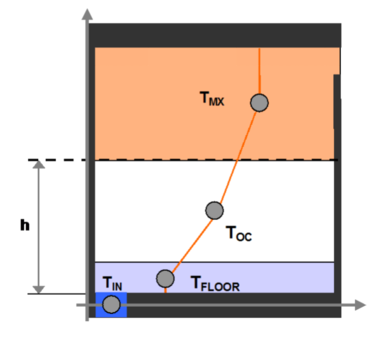
\includegraphics[width=0.9\textwidth, height=0.9\textheight, keepaspectratio=true]{media/image080.png}
\caption{Schematic representation of the three temperature points and temperature gradients \protect \label{fig:schematic-representation-of-the-three}}
\end{figure}

The following fields are used to define an instance of the `UCSD Displacement Ventilation Model Controls' object.

\subsubsection{Inputs}\label{inputs-8-020}

\paragraph{Field: Zone Name}\label{field-zone-name-4-005}

This field provides the unique name of a zone described elsewhere in the file. A single instance of the `UCSD Displacement Ventilation Model Controls' object is needed for each zone that is to be modeled using this method.

\paragraph{Field: Gain Distribution Schedule Name}\label{field-gain-distribution-schedule-name}

This field specifies the unique name of schedule defined elsewhere in the input file. The schedule values are the fractions of the convective portion of the internal gains in the occupied subzone that remain in the occupied subzone. The remainder of the convective portion of the internal gains in the occupied subzone enters the plumes and is carried to the upper subzone. The types of internal gains that are assumed to be located in the occupied subzone are:

\begin{itemize}
\item
  people
\item
  task lights
\item
  electric equipment
\item
  gas equipment
\item
  hot water equipment
\item
  steam equipment
\item
  other equipment
\item
  baseboard heat
\end{itemize}

Types of internal gains that are assumed to be in the upper subzone are:

\begin{itemize}
\item
  general lights
\item
  tubular daylighting devices
\item
  high temperature radiant heaters
\end{itemize}

The schedule values should be between 0 and 1. A value of 1 means that all the convection gains from equipment, task lights and people are dispersed in the lower occupied subzone. Conversely a value of 0 puts all the lower subzone convective gains into the plumes rising into the upper well-mixed subzone.

\paragraph{Field: Number of Plumes per Occupant}\label{field-number-of-plumes-per-occupant}

This field specifies number of plumes per occupant. Plumes are associated with localized sources of convective heat gain from people and equipment. For example, a value of 2.0 would be used if each occupant has a computer that generates a separate plume that does not merge with the plume from the occupant in the lower, occupied, subzone.

\paragraph{Field: Thermostat Height}\label{field-thermostat-height-1}

This field is the height in meters of the thermostat/temperature control sensor above the floor.

\paragraph{Field: Comfort Height}\label{field-comfort-height}

The height in meters above the floor at which air temperature is calculated for comfort purposes. The air temperature at this height is used in calculating the available measures of comfort: Fanger, Pierce, KSU, CoolingEffectASH55 or AnkleDraftASH55. The default is 1.1 meters.

\paragraph{Field: Temperature Difference Threshold for Reporting}\label{field-temperature-difference-threshold-for-reporting}

This field specifies a minimum temperature difference between the upper mixed subzone and the occupied subzone that will be used to trigger whether or not the displacement ventilation auxiliary outputs will be calculated. These outputs are \emph{Room Air Zone Transition Height}, \emph{Room Air Zone Recommended Minimum Flow Fraction}, \emph{Room Air Zone Average Temperature Gradient} and \emph{Room Air Zone Maximum Temperature Gradient}. They are set to negative values when the temperature difference is less than the threshold and the output \emph{Room Air Zone Is Mixed Status} is set to 1.

The value should be greater than or equal to zero and is in units of degrees Centigrade. The default value is 0.4 degrees C.

An example input:

\begin{lstlisting}

RoomAirSettings:ThreeNodeDisplacementVentilation,
      ZONE ONE,  !- Zone Name
      Constant - .2,  !- Gain Distribution Schedule Name
       1,  !- Number of Plumes per Occupant
        ,  !- Thermostat Height
        ,  !- Comfort Height
      .3;  !- Temp. Difference Threshold for Displacement Ventilation
\end{lstlisting}

\subsubsection{Outputs}\label{roomairsettingsthreenodedisplacementventilation-outputs}

\begin{itemize}
\item
  HVAC,Average,Room Air Zone Mixed Subzone Temperature {[}C{]}
\item
  HVAC,Average,Room Air Zone Occupied Subzone Temperature {[}C{]}
\item
  HVAC,Average,Room Air Zone Floor Subzone Temperature {[}C{]}
\item
  HVAC,Average,Room Air Zone Transition Height {[}m{]}
\item
  HVAC,Average,Room Air Zone Recommended Minimum Flow Fraction
\item
  HVAC,Average,Room Air Zone Is Mixed Status
\item
  HVAC,Average,Room Air Zone Average Temperature Gradient {[}K/m{]}
\item
  HVAC,Average,Room Air Zone Maximum Temperature Gradient {[}K/m{]}
\item
  HVAC,Average,Room Air Zone Thermal Comfort Effective Air Temperature {[}C{]}
\item
  HVAC,Average,Room Air Zone Thermostat Temperature {[}C{]}
\end{itemize}

\paragraph{Room Air Zone Mixed Subzone Temperature {[}C{]}}\label{room-air-zone-mixed-subzone-temperature-c}

The temperature of the upper well-mixed subzone in degrees C.

\paragraph{Room Air Zone Occupied Subzone Temperature {[}C{]}}\label{room-air-zone-occupied-subzone-temperature-c}

The average temperature of the lower, stratified, occupied subzone in degrees C.

\paragraph{Room Air Zone Floor Subzone Temperature {[}C{]}}\label{room-air-zone-floor-subzone-temperature-c}

The temperature of the region near the floor in degrees C.

\paragraph{Room Air Zone Transition Height {[}m{]}}\label{room-air-zone-transition-height-m}

The height above the floor, in meters, of the boundary between the lower occupied subzone and the upper well-mixed subzone.

\paragraph{Room Air Zone Recommended Minimum Flow Fraction {[]}}\label{room-air-zone-recommended-minimum-flow-fraction}

The ratio of the minimum recommended flow rate to the actual flow rate. Here flow rate means the sum of infiltration, ventilation, mixing and system air flow rates. The minimum flow is the flow needed to establish the boundary between the occupied and mixed subzones at 1.5 meters.

\paragraph{Room Air Zone Is Mixed Status {[]}}\label{room-air-zone-is-mixed-status}

An integer flag that indicates whether the zone is mixed (single node well-mixed zone model used) or stratified (UCSD DV model used). The value 1 means well-mixed; 0 means stratified.

\paragraph{Room Air Zone Average Temperature Gradient {[}K/m{]}}\label{room-air-zone-average-temperature-gradient-km}

The temperature gradient between the middle of the floor region and the middle of the well-mixed upper subzone in degrees Kelvin per meter.

\paragraph{Room Air Zone Maximum Temperature Gradient {[}K/m{]}}\label{room-air-zone-maximum-temperature-gradient-km}

The maximum of the temperature gradient between the middle of the floor region and the middle of the occupied subzone and the temperature gradient between the middle of the occupied subzone and the middle of the well-mixed subzone. The gradient is in degrees Kelvin per meter.

\paragraph{Room Air Zone Thermal Comfort Effective Air Temperature {[}C{]}}\label{room-air-zone-thermal-comfort-effective-air-temperature-c}

The temperature at the user specified comfort height in degrees C.

\paragraph{Room Air Zone Thermostat Temperature {[}C{]}}\label{room-air-zone-thermostat-temperature-c}

The temperature at the height of the thermostat (specified by user input) in degrees C.

\subsection{RoomAirSettings:CrossVentilation}\label{roomairsettingscrossventilation}

The UCSD Cross Ventilation Room Air Model provides a simple model for heat transfer and temperature prediction in cross ventilated rooms. Cross Ventilation (CV) is common in many naturally ventilated buildings, with air flowing through windows, open doorways and large internal apertures across rooms and corridors in the building.

The CV model is used in EnergyPlus in the context of natural ventilation simulations using the AirflowNetwork airflow prediction model. Typical CV room flows are characterized by two clearly distinguishable flow regions that have different airflow velocities and temperature:

\begin{itemize}
\item
  Jet regions in front of the inflow windows
\item
  Recirculation regions in the portions of the room that are not directly in front of the windows.
\end{itemize}

Each inflow aperture has one jet region while the recirculation regions are treated as a whole, with a single temperature and characteristic velocity. The default EnergyPlus perfectly mixed single temperature node room air approach is not suitable for these partially mixed flows. The proposed CV model uses multiple nodes with distinct air temperature and airflow velocity (one node for the recirculations plus one additional node for each inflow aperture).

\begin{figure}[hbtp] % fig 46
\centering
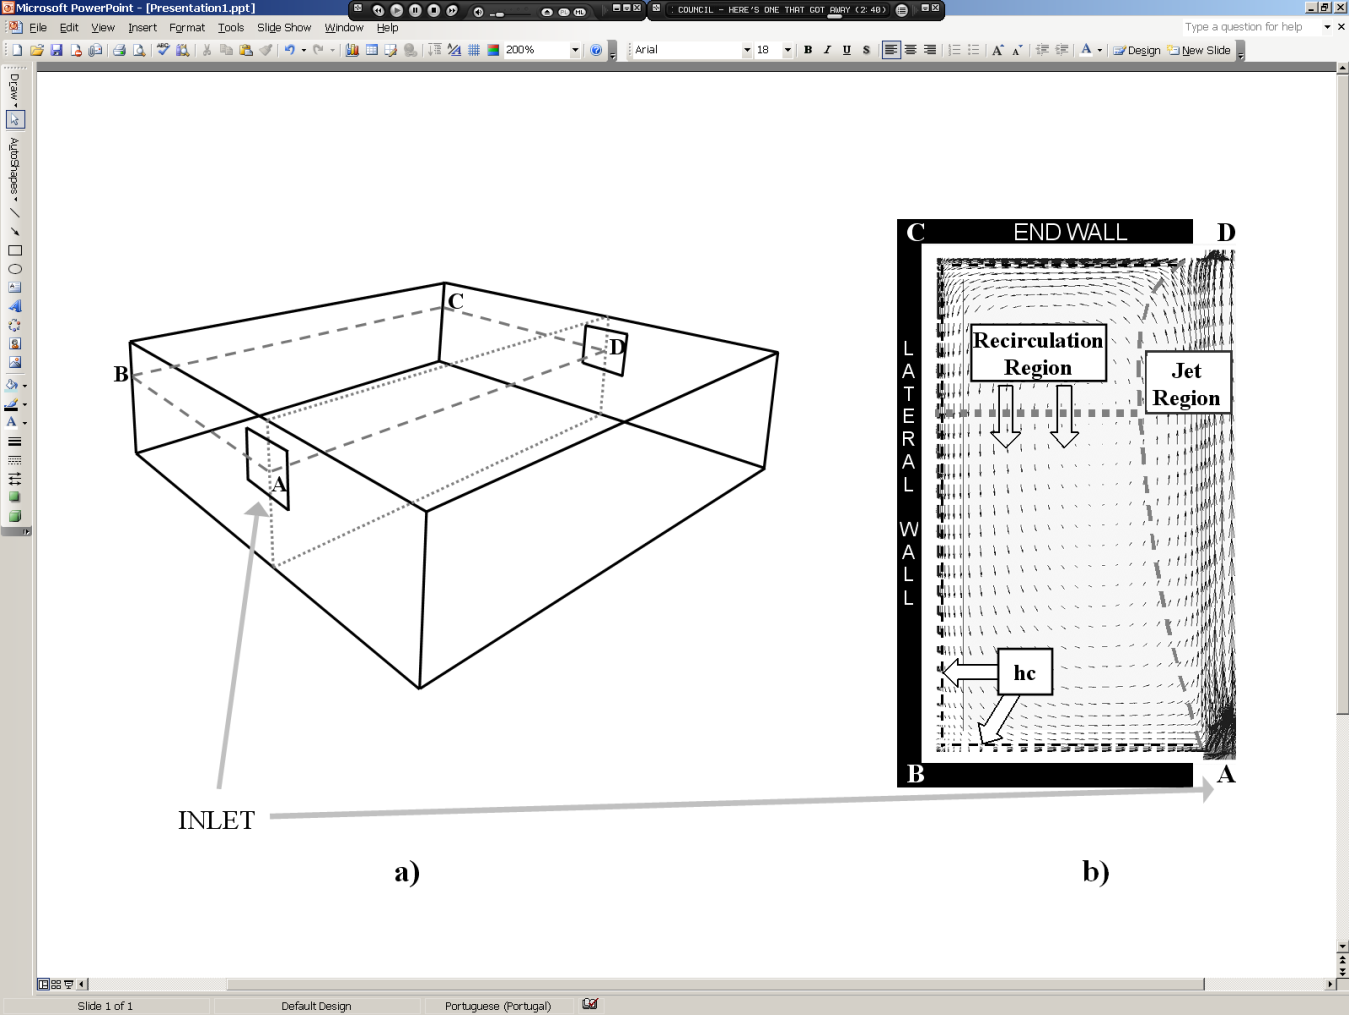
\includegraphics[width=0.9\textwidth, height=0.9\textheight, keepaspectratio=true]{media/image081.png}
\caption{Schematic representation of room air geometry a) schematic representation of a room geometry that generates cross ventilation airflow. b) the proposed model distinguishes two regions in the flow: jet and recirculation (shown here in a CFD simulation of one half of a symmetrical room). \protect \label{fig:schematic-representation-of-room-air-geometry}}
\end{figure}

\begin{figure}[hbtp] % fig 47
\centering
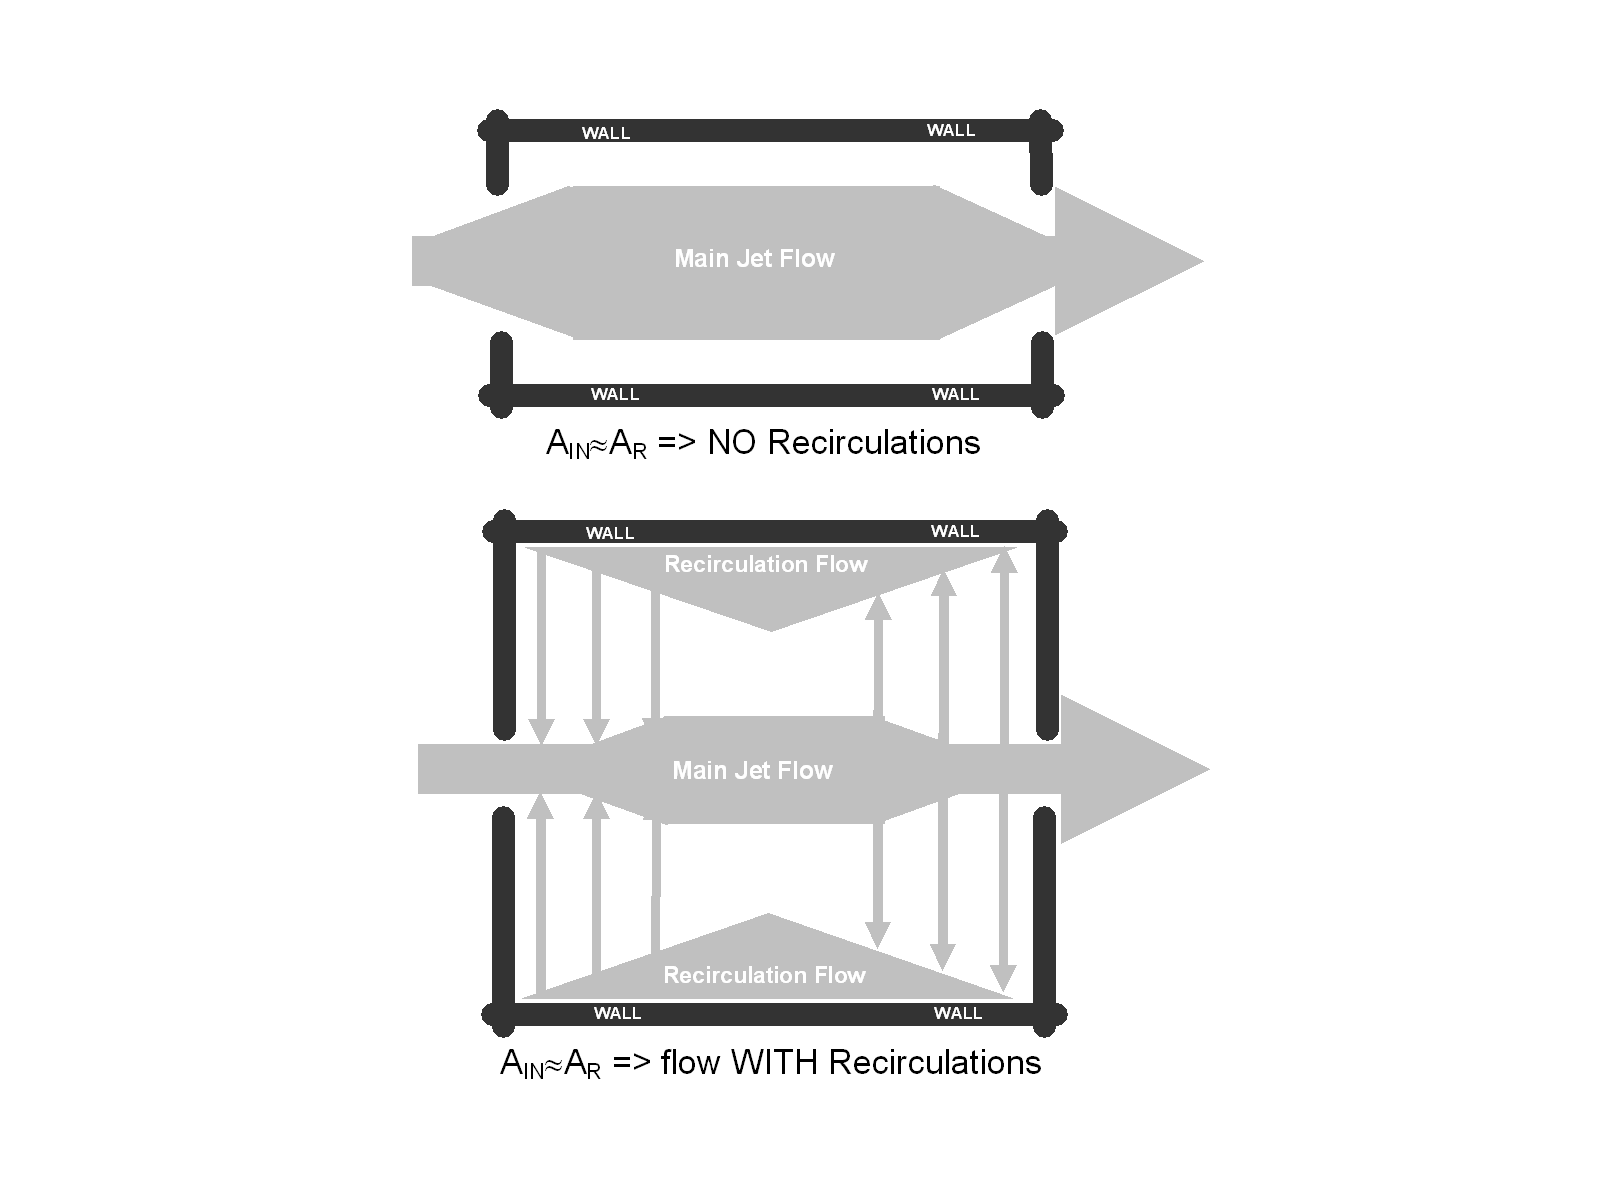
\includegraphics[width=0.9\textwidth, height=0.9\textheight, keepaspectratio=true]{media/image082.png}
\caption{Schematic top view --- possible airflow patterns in cross-ventilation. \protect \label{fig:schematic-top-view-possible-airflow-patterns}}
\end{figure}

The following fields are used to define an instance of the `UCSD Cross Ventilation Model Controls' object.

\subsubsection{Inputs}\label{inputs-9-018}

\paragraph{Field: Zone Name}\label{field-zone-name-5-004}

This field provides the name of the zone to which this object applies. A single instance of the `UCSD Cross Ventilation Model Controls' object is needed for each zone modeled using this method.

\paragraph{Field: Gain Distribution Schedule Name}\label{field-gain-distribution-schedule-name-1}

This field specifies the unique name of schedule defined elsewhere in the input file. The schedule values define the fractions of the convective portion of the internal gains in the jet and recirculation regions.

The schedule values should be between 0 and 1. A value of 1 means that all the convective gains are dispersed in the jet region. Conversely a value of 0 puts all the convective gains into the recirculation region.

\paragraph{Field: Airflow Region Used for Thermal Comfort Evaluation}\label{field-airflow-region-used-for-thermal-comfort-evaluation}

Required field whenever thermal comfort is predicted. Defines air temperature and mean airflow velocity that will be used in the Fanger model. Conditions must refer to one of the two regions defined in the model: jet or recirculation.

Possible choices: Jet or Recirculation.

\subsubsection{Outputs}

\begin{itemize}
\item
  Zone,Average,Room Air Zone Jet Region Temperature {[}C{]}
\item
  Zone,Average,Room Air Zone Recirculation Region Temperature {[}C{]}
\item
  Zone,Average,Room Air Zone Jet Region Average Air Velocity {[}m/s{]}
\item
  Zone,Average,Room Air Zone Recirculation Region Average Air Velocity {[}m/s{]}
\item
  Zone,Average,Room Air Window Jet Region Average Air Velocity {[}m/s{]}
\item
  Zone,Average,Room Air Zone Recirculation and Inflow Rate Ratio
\item
  Zone,Average,Room Air Zone Inflow Opening Area {[}m2{]}
\item
  Zone,Average,Room Air Zone Room Length {[}m{]}
\item
  Zone,Average,Room Air Zone Is Mixing Status
\item
  Zone,Average,Room Air Zone Is Recirculating Status
\end{itemize}

\paragraph{Room Air Zone Jet Region Temperature {[}C{]}}\label{room-air-zone-jet-region-temperature-c}

Average air temperature in the jet region of the flow in degrees C. If there is more than one inflow window this output will be the inflow-area-weighted average of the jet region temperature.

\paragraph{Room Air Zone Recirculation Region Temperature {[}C{]}}\label{room-air-zone-recirculation-region-temperature-c}

Average air temperature in the recirculation region of the flow in degrees C.

\paragraph{Room Air Zone Jet Region Average Air Velocity {[}m/s{]}}\label{room-air-zone-jet-region-average-air-velocity-ms}

Average airflow velocity in the jet region of the flow in meters per second. If there is more than one inflow window this output will be the inflow area weighted area of the jet inflow velocities.

\paragraph{Room Air Window Jet Region Average Air Velocity {[}m/s{]}}\label{room-air-window-jet-region-average-air-velocity-ms}

Average airflow velocity in the jet region in front of the window, in meters per second.

\paragraph{Room Air Zone Recirculation Region Average Air Velocity {[}m/s{]}}\label{room-air-zone-recirculation-region-average-air-velocity-ms}

Average airflow velocity in the recirculation region of the flow in meters per second.

\paragraph{Room Air Zone Recirculation and Inflow Rate Ratio {[]}}\label{room-air-zone-recirculation-and-inflow-rate-ratio}

Ratio between airflow rate in the recirculation regions and the total inflow rate, non-dimensional.

\paragraph{Room Air Zone Inflow Opening Area {[}m2{]}}\label{room-air-zone-inflow-opening-area-m2}

Area of the inflow aperture in square meters. This area can change due to variation in wind direction (as inflow aperture changes) or variations in the opening schedule.

\paragraph{Room Air Zone Room Length {[}m{]}}\label{room-air-zone-room-length-m}

Length of the room along the cross ventilation direction, in meters.

\paragraph{Room Air Zone Is Mixing Status {[]}}\label{room-air-zone-is-mixing-status}

An integer flag that indicates whether the zone is mixed (single node well-mixed zone model used) or significant momentum conservation is occurring (UCSD CV model used). The value 1 means well-mixed; 0 means cross ventilation is present. Transition to mixed flow can occur due to three mechanism: reduction in inflow velocity, reduction in inflow aperture area and dominance of buoyancy effects. A value of 1 is yes, a value of 0 is no.

\paragraph{Room Air Zone Is Recirculating Status {[]}}\label{room-air-zone-is-recirculating-status}

An integer flag that indicates whether recirculations are present in the flow. A cross ventilation flow does not have recirculations whenever the inflow area is similar to the room cross section area (such as airflow in a typical corridor). A value of 1 is yes, a value of 0 is no.

\subsection{RoomAirSettings:UnderFloorAirDistributionInterior}\label{roomairsettingsunderfloorairdistributioninterior}

This model is applicable to interior spaces that are served by an underfloor air distribution system. The dominant sources of heat gain should be from people, equipment, and other localized sources located in the occupied part of the room. The model should be used with caution in zones which have large heat gains or losses through exterior walls or windows or which have considerable direct solar gain. The model predicts two temperatures in the room:

\begin{itemize}
\item
  An occupied subzone temperature (T\(_{\rm{OC}}\)), representing the temperature in the region between the floor and the boundary of the upper subzone.
\item
  An upper subzone temperature (T\(_{\rm{MX}}\)) essential for overall energy budget calculations and for modeling comfort effects of the upper layer temperature.
\end{itemize}

The following fields are used to define an instance of the `UCSD UFAD Interior Model Controls' object.

\subsubsection{Inputs}\label{inputs-2016-06-17-0938}

\paragraph{Field: Zone Name}\label{field-zone-name-6-003}

This field provides the unique name of a zone described elsewhere in the file. A single instance of the `RoomAirSettings:UnderFloorAirDistributionInterior' object is needed for each zone that is to be modeled using this method.

\paragraph{Field: Number of Diffusers}\label{field-number-of-diffusers}

The total number of diffusers in this zone. This field can allowed to Autocalculate (in which case it is set to the design occupancy level; i.e., number of people). If the design occupancy is low or zero but there are still heat sources that could generate buoyancy driven plumes, the user should input a value based on the design supply air flow rate of the zone and the design flow rate of an individual diffuser. In the absence of any other information, divide the zone area by 100 ft\(^{2}\). The default for this field is Autocalculate.

\paragraph{Field: Power per Plume}\label{field-power-per-plume}

The power in watts incorporated in a buoyancy driven thermal plume. Normally we assume all the loads of a workstation create a single plume so that this represents the convective heat gain from a workstation -- 1 person, 1 computer terminal, plus any task lighting. A typical value would be 220 watts. However, the model assumes an ``equivalent'' plume derived from the zone extraction rate normalized to the number of workstations/occupants. This field should be allowed to default -- the program will calculate a value based upon the occupancy and the extraction rate. The default is Autocalculate.

\paragraph{Field: Design Effective Area of Diffuser}\label{field-design-effective-area-of-diffuser}

This is the design air flow opening area in square meters of a single diffuser. The default value depends on the diffuser type. For swirl diffusers it is 0075 m\(^{2}\), for variable area diffusers 0.035 m\(^{2}\), for horizontal swirl diffusers 0.006 m\(^{2}\), and for linear bar grilles 0.03 m\(^{2}\). The default is \emph{Autocalculate}..

\paragraph{Field: Diffuser Slot Angle from Vertical}\label{field-diffuser-slot-angle-from-vertical}

This input describes the angle at which air emerges from the diffusers. It should be the angle in degrees between the vertical and the diffuser slots. The defaults depend on the diffuser type: for swirl diffusers it is 28 degrees, for variable area diffusers 45 degrees, for DV diffusers 73 degrees, and for linear bar grilles 15 degrees.

\paragraph{Field: Thermostat Height}\label{field-thermostat-height-2}

This field is the height in meters of the thermostat/temperature control sensor above the floor. The default is 1.2 meters.

\paragraph{Field: Comfort Height}\label{field-comfort-height-1}

The height in meters above the floor at which air temperature is calculated for comfort purposes. The air temperature at this height is used in calculating the available measures of comfort: Fanger, Pierce, KSU, CoolingEffectASH55 or AnkleDraftASH55. The default is 1.1 meters.

\paragraph{Field: Temperature Difference Threshold for Reporting}\label{field-temperature-difference-threshold-for-reporting-1}

This field specifies a minimum temperature difference between the upper subzone and the occupied subzone that will be used to trigger whether or not the UFAD auxiliary outputs will be calculated. These outputs are \emph{Room Air Zone Transition Height} and \emph{Room Air Zone Average Temperature Gradient}. They are set to zero when the temperature difference is less than the threshold and the output \emph{Room Air Zone Is Mixed Status} is set to 1.

The value should be greater than or equal to zero and is in units of degrees Centigrade. The default value is 0.4 degrees C.

\paragraph{Field: Diffuser Type}\label{field-diffuser-type}

The choices for this alpha field are \textbf{Swirl} \textbar{} \textbf{VariableArea} \textbar{} \textbf{HorizontalSwirl \textbar{} LinearBarGrille \textbar{} Custom.} The swirl and displacement diffusers are fixed area diffusers. The variable area diffusers maintain an approximately constant exit velocity. Linear bar grilles are normally used in exterior zones and are fixed area diffusers. Custom is used to signify that the user intends to input the coefficients A -- E (see below) rather than let the program set the coefficients based on diffuser type. The default is \emph{Swirl}.

\paragraph{Field: Transition Height}\label{field-transition-height}

An optional field to allow the user to specify the transition height (meters above floor) rather than have the program calculate it. The default is 1.7 meters.

\paragraph{Field: Coefficient A}\label{field-coefficient-a}

The coefficient A in the formula: Kc = A*Gamma**B + C + D*Gamma + E*Gamma**2. Gamma is a variable that characterizes the amount of stratification in a UFAD zone. Kc is the fraction of the total internal convective heat gain that is assigned to the lower (occupied) subzone. The coefficients in the formula are defaulted based upon diffuser type. A user would normally allow this field to default. The default is \emph{autocalculate}.

\paragraph{Field: Coefficient B}\label{field-coefficient-b}

The coefficient B in the formula: Kc = A*Gamma**B + C + D*Gamma + E*Gamma**2. Gamma is a variable that characterizes the amount of stratification in a UFAD zone. Kc is the fraction of the total internal convective heat gain that is assigned to the lower (occupied) subzone. The coefficients in the formula are defaulted based upon diffuser type. A user would normally allow this field to default. The default is \emph{autocalculate}.

\paragraph{Field: Coefficient C}\label{field-coefficient-c}

The coefficient C in the formula: Kc = A*Gamma**B + C + D*Gamma + E*Gamma**2. Gamma is a variable that characterizes the amount of stratification in a UFAD zone. Kc is the fraction of the total internal convective heat gain that is assigned to the lower (occupied) subzone. The coefficients in the formula are defaulted based upon diffuser type. A user would normally allow this field to default. The default is \emph{autocalculate}.

\paragraph{Field: Coefficient D}\label{field-coefficient-d}

The coefficient D in the formula: Kc = A*Gamma**B + C + D*Gamma + E*Gamma**2. Gamma is a variable that characterizes the amount of stratification in a UFAD zone. Kc is the fraction of the total internal convective heat gain that is assigned to the lower (occupied) subzone. The coefficients in the formula are defaulted based upon diffuser type. A user would normally allow this field to default. The default is \emph{autocalculate}.

\paragraph{Field: Coefficient E}\label{field-coefficient-e}

The coefficient E in the formula: Kc = A*Gamma**B + C + D*Gamma + E*Gamma**2. Gamma is a variable that characterizes the amount of stratification in a UFAD zone. Kc is the fraction of the total internal convective heat gain that is assigned to the lower (occupied) subzone. The coefficients in the formula are defaulted based upon diffuser type. A user would normally allow this field to default. The default is \emph{autocalculate}.

An example input is:

\begin{lstlisting}

  RoomAirModelType,
      SPACE5-1 RoomAir Model,  !- Name
      SPACE5-1,                !- Zone Name
      UnderFloorAirDistributionInterior,  !- Room-Air Modeling Type
      DIRECT;                  !- Air Temperature Coupling Strategy

  RoomAirSettings:UnderFloorAirDistributionInterior,
      SPACE5-1,                !- Zone Name
      Autocalculate,           !- Number of Diffusers
      Autocalculate,           !- Power per Plume
      Autocalculate,           !- Design Effective Area of Diffuser {m2}
      Autocalculate,           !- Diffuser Slot Angle from Vertical {deg}
      ,                        !- Thermostat Height {m}
      ,                        !- Comfort Height {m}
      0.001,         !- Temperature Difference Threshold for Reporting {deltaC}
      Swirl,                   !- Diffuser Type
      1.7,                     !- Transition Height {m}
      Autocalculate,           !- Coefficient A
      Autocalculate,           !- Coefficient B
      Autocalculate,           !- Coefficient C
      Autocalculate,           !- Coefficient D
     Autocalculate;           !- Coefficient E
\end{lstlisting}

\subsubsection{Outputs}\label{roomairsettingsunderfloorairdistributioninterior-outputs}

\begin{itemize}
\item
  HVAC,Average,Room Air Zone Mixed Subzone Temperature {[}C{]}
\item
  HVAC,Average,Room Air Zone Occupied Subzone Temperature {[}C{]}
\item
  HVAC,Average,Room Air Zone Transition Height {[}m{]}
\item
  HVAC,Average,Room Air Zone Is Mixed Status {[]}
\item
  HVAC,Average,Room Air Zone Average Temperature Gradient {[}K/m{]}
\item
  HVAC,Average,Room Air Zone Effective Comfort Air Temperature {[}C{]}
\item
  HVAC,Average,Room Air Zone Thermostat Temperature {[}C{]}
\item
  HVAC,Average,Room Air Zone Transition Height Gamma Value {[]}
\item
  HVAC,Average,Room Air Zone Plume Heat Transfer Rate {[}W{]}
\item
  HVAC,Average,Room Air Zone Temperature Stratification Fraction {[]}
\end{itemize}

\paragraph{Room Air Zone Mixed Subzone Temperature {[}C{]}}\label{room-air-zone-mixed-subzone-temperature-c-1}

The temperature of the upper subzone in degrees C.

\paragraph{Room Air Zone Occupied Subzone Temperature {[}C{]}}\label{room-air-zone-occupied-subzone-temperature-c-1}

The temperature of the lower, occupied subzone in degrees C.

\paragraph{Room Air Zone Transition Height {[}m{]}}\label{room-air-zone-transition-height-m-1}

The height above the floor, in meters, of the boundary between the lower occupied subzone and the upper subzone..

\paragraph{Room Air Zone Is Mixed Status {[]}}\label{room-air-zone-is-mixed-status-1}

An integer flag that indicates whether the zone is mixed (single node well-mixed zone model used) or stratified (UCSD UFI model used). The value 1 means well-mixed; 0 means stratified.

\paragraph{Room Air Zone Average Temperature Gradient {[}K/m{]}}\label{room-air-zone-average-temperature-gradient-km-1}

The temperature gradient between the middle of the occupied subzone and the middle of the upper subzone in degrees Kelvin per meter.

\paragraph{Room Air Zone Effective Comfort Air Temperature {[}C{]}}\label{room-air-zone-effective-comfort-air-temperature-c}

The temperature at the user specified comfort height in degrees C.

\paragraph{Room Air Zone Thermostat Temperature {[}C{]}}\label{room-air-zone-thermostat-temperature-c-1}

The temperature at the height of the thermostat (specified by user input) in degrees C.

\paragraph{Room Air Zone Transition Height Gamma Value {[]}}\label{room-air-zone-transition-height-gamma-value}

Value of gamma -- a dimensionless ``height'' used in calculating the transition height. Lower values of gamma indicate increased stratification, higher values less. Generally the values should be between 2 and 30.

\paragraph{Room Air Zone Plume Heat Transfer Rate {[}W{]}}\label{room-air-zone-plume-heat-transfer-rate-w}

The heat in watts driving the plumes in the occupied subzone.

\paragraph{Room Air Zone Temperature Stratification Fraction {[]}}\label{room-air-zone-temperature-stratification-fraction}

This output, (Phi) is a measure of temperature stratification in the space. It is the difference between the occupied subzone temperature and the supply temperature divided by difference between the return temperature and the supply temperature. Technically it is equal to Kc. As phi approaches 1, the space is fully mixed. As phi approaches 0, the space becomes fully stratified. Expressed as an equation:

\begin{equation}
  \frac{T_{occ} - T_{sup}}{T_{ret} - T_{sup}}
\end{equation}

\subsection{RoomAirSettings:UnderFloorAirDistributionExterior}\label{roomairsettingsunderfloorairdistributionexterior}

This model is applicable to exterior spaces that are served by an underfloor air distribution system. The dominant sources of heat gain should be from people, equipment, and other localized sources located in the occupied part of the room, as well as convective gain coming from a warm window. The model predicts two temperatures in the room:

\begin{itemize}
\item
  An occupied subzone temperature (T\(_{\rm{OC}}\)), representing the temperature in the region between the floor and the boundary of the upper subzone..
\item
  An upper subzone temperature (T\(_{\rm{MX}}\)) essential for overall energy budget calculations and for modeling comfort effects of the upper layer temperature.
\end{itemize}

The following fields are used to define an instance of the `UCSD UFAD Exterior Model Controls' object.

\subsubsection{Inputs}\label{inputs-11-016}

\paragraph{Field: Zone Name}\label{field-zone-name-7-003}

This field provides the unique name of a zone described elsewhere in the file. A single instance of the `RoomAirSettings:UnderFloorAirDistributionExterior' object is needed for each zone that is to be modeled using this method.

\paragraph{Field: Number of Diffusers}\label{field-number-of-diffusers-1}

The total number of diffusers in this zone. This field can allowed to Autocalculate (in which case it is set to the design occupancy level; i.e., number of people). If the design occupancy is low or zero but there are still heat sources that could generate buoyancy driven plumes, the user should input a value based on the design supply air flow rate of the zone and the design flow rate of an individual diffuser. In the absence of any other information, divide the zone area by 100 ft\(^{2}\). The default for this field is Autocalculate.

\paragraph{Field: Power per Plume}\label{field-power-per-plume-1}

The power in watts incorporated in a buoyancy driven thermal plume. Normally we assume all the loads of a workstation create a single plume so that this represents the convective heat gain from a workstation -- 1 person, 1 computer terminal, plus any task lighting. A typical value would be 220 watts. However, the model assumes an ``equivalent'' plume derived from the zone extraction rate normalized to the number of workstations/occupants. This field should be allowed to default -- the program will calculate a value based upon the occupancy and the extraction rate. The default is Autocalculate.

\paragraph{Field: Design Effective Area of Diffuser}\label{field-design-effective-area-of-diffuser-1}

This is the design air flow opening area in square meters of a single diffuser. The default value depends on the diffuser type. For swirl diffusers it is 0075 m\(^{2}\), for variable area diffusers 0.035 m\(^{2}\), for horizontal swirl diffusers 0.006 m\(^{2}\), and for linear bar grilles 0.03 m\(^{2}\). The default is \emph{Autocalculate}..

\paragraph{Field: Diffuser Slot Angle from Vertical}\label{field-diffuser-slot-angle-from-vertical-1}

This input describes the angle at which air emerges from the diffusers. It should be the angle in degrees between the vertical and the diffuser slots. The defaults depend on the diffuser type: for swirl diffusers it is 28 degrees, for variable area diffusers 45 degrees, for DV diffusers 73 degrees, and for linear bar grilles 15 degrees.

\paragraph{Field: Thermostat Height}\label{field-thermostat-height-3}

This field is the height in meters of the thermostat/temperature control sensor above the floor. The default is 1.2 meters.

\paragraph{Field: Comfort Height}\label{field-comfort-height-2}

The height in meters above the floor at which air temperature is calculated for comfort purposes. The air temperature at this height is used in calculating the available measures of comfort: Fanger, Pierce, KSU, CoolingEffectASH55 or AnkleDraftASH55. The default is 1.1 meters.

\paragraph{Field: Temperature Difference Threshold for Reporting}\label{field-temperature-difference-threshold-for-reporting-2}

This field specifies a minimum temperature difference between the upper subzone and the occupied subzone that will be used to trigger whether or not the UFAD auxiliary outputs will be calculated. These outputs are \emph{Room Air Zone Transition Height} and \emph{Room Air Zone Average Temperature Gradient}. They are set to zero when the temperature difference is less than the threshold and the output \emph{Room Air Zone Is Mixed Status} is set to 1.

The value should be greater than or equal to zero and is in units of degrees Centigrade. The default value is 0.4 degrees C.

The value should be greater than or equal to zero and is in units of degrees Centigrade. The default value is 0.4 degrees C.

\paragraph{Field: Diffuser Type}\label{field-diffuser-type-1}

The choices for this alpha field are \textbf{Swirl} \textbar{} \textbf{VariableArea} \textbar{} \textbf{HorizontalSwirl \textbar{} LinearBarGrille \textbar{} Custom.} The swirl and displacement diffusers are fixed area diffusers. The variable area diffusers maintain an approximately constant exit velocity. Linear bar grilles are normally used in exterior zones and are fixed area diffusers. Custom is used to signify that the user intends to input the coefficients A -- E (see below) rather than let the program set the coefficients based on diffuser type. The default is \emph{Swirl}.

\paragraph{Field: Transition Height}\label{field-transition-height-1}

An optional field to allow the user to specify the transition height (meters above floor) rather than have the program calculate it. The default is 1.7 meters.

\paragraph{Field: Coefficient A}\label{field-coefficient-a-1}

The coefficient A in the formula: Kc = A*Gamma**B + C + D*Gamma + E*Gamma**2. Gamma is a variable that characterizes the amount of stratification in a UFAD zone. Kc is the fraction of the total internal convective heat gain that is assigned to the lower (occupied) subzone. The coefficients in the formula are defaulted based upon diffuser type. A user would normally allow this field to default. The default is \emph{autocalculate}.

\paragraph{Field: Coefficient B}\label{field-coefficient-b-1}

The coefficient B in the formula: Kc = A*Gamma**B + C + D*Gamma + E*Gamma**2. Gamma is a variable that characterizes the amount of stratification in a UFAD zone. Kc is the fraction of the total internal convective heat gain that is assigned to the lower (occupied) subzone. The coefficients in the formula are defaulted based upon diffuser type. A user would normally allow this field to default. The default is \emph{autocalculate}.

\paragraph{Field: Coefficient C}\label{field-coefficient-c-1}

The coefficient C in the formula: Kc = A*Gamma**B + C + D*Gamma + E*Gamma**2. Gamma is a variable that characterizes the amount of stratification in a UFAD zone. Kc is the fraction of the total internal convective heat gain that is assigned to the lower (occupied) subzone. The coefficients in the formula are defaulted based upon diffuser type. A user would normally allow this field to default. The default is \emph{autocalculate}.

\paragraph{Field: Coefficient D}\label{field-coefficient-d-1}

The coefficient D in the formula: Kc = A*Gamma**B + C + D*Gamma + E*Gamma**2. Gamma is a variable that characterizes the amount of stratification in a UFAD zone. Kc is the fraction of the total internal convective heat gain that is assigned to the lower (occupied) subzone. The coefficients in the formula are defaulted based upon diffuser type. A user would normally allow this field to default. The default is \emph{autocalculate}.

\paragraph{Field: Coefficient E}\label{field-coefficient-e-1}

The coefficient E in the formula: Kc = A*Gamma**B + C + D*Gamma + E*Gamma**2. Gamma is a variable that characterizes the amount of stratification in a UFAD zone. Kc is the fraction of the total internal convective heat gain that is assigned to the lower (occupied) subzone. The coefficients in the formula are defaulted based upon diffuser type. A user would normally allow this field to default. The default is \emph{autocalculate}.

An example input is:

\begin{lstlisting}
RoomAirSettings:UnderFloorAirDistributionExterior,
      SPACE1-1,                !- Zone Name
      Autocalculate,           !- Number of Diffusers per Zone
      Autocalculate,           !- Power per Plume
      Autocalculate,           !- Design Effective Area of Diffuser {m2}
      Autocalculate,           !- Diffuser Slot Angle from Vertical {deg}
      ,                        !- Thermostat Height {m}
      ,                        !- Comfort Height {m}
      0.001,                   !- Temperature Difference Threshold for Reporting {deltaC}
      LinearBarGrille,         !- Diffuser Type
      1.7,                     !- Transition Height {m}
      Autocalculate,           !- Coefficient A
      Autocalculate,           !- Coefficient B
      Autocalculate,           !- Coefficient C
      Autocalculate,           !- Coefficient D
      Autocalculate;           !- Coefficient E
\end{lstlisting}

\subsubsection{Outputs}\label{roomairsettingsunderfloorairdistributionexterior-outputs}

\begin{itemize}
\item
  HVAC,Average,Room Air Zone Mixed Subzone Temperature {[}C{]}
\item
  HVAC,Average,Room Air Zone Occupied Subzone Temperature {[}C{]}
\item
  HVAC,Average,Room Air Zone Transition Height {[}m{]}
\item
  HVAC,Average,Room Air Zone Is Mixed Status {[]}
\item
  HVAC,Average,Room Air Zone Average Temperature Gradient {[}K/m{]}
\item
  HVAC,Average,Room Air Zone Effective Comfort Air Temperature {[}C{]}
\item
  HVAC,Average,Room Air Zone Thermostat Temperature {[}C{]}
\item
  HVAC,Average,Room Air Zone Transition Height Gamma Value {[]}
\item
  HVAC,Average,Room Air Zone Plume Heat Transfer Rate {[}W{]}
\item
  HVAC,Average,Room Air Zone Window Plume Heat Transfer Rate {[}W{]}
\item
  HVAC,Average,Room Air Zone Temperature Stratification Fraction {[]}
\end{itemize}

\paragraph{Room Air Zone Mixed Subzone Temperature {[}C{]}}\label{room-air-zone-mixed-subzone-temperature-c-1-2}

The temperature of the upper subzone in degrees C.

\paragraph{Room Air Zone Occupied Subzone Temperature {[}C{]}}\label{room-air-zone-occupied-subzone-temperature-c-1-2}

The temperature of the lower, occupied subzone in degrees C.

\paragraph{Room Air Zone Transition Height {[}m{]}}\label{room-air-zone-transition-height-m-1-2}

The height above the floor, in meters, of the boundary between the lower occupied subzone and the upper subzone..

\paragraph{Room Air Zone Is Mixed Status {[]}}\label{room-air-zone-is-mixed-status-1-2}

An integer flag that indicates whether the zone is mixed (single node well-mixed zone model used) or stratified (UCSD UFE model used). The value 1 means well-mixed; 0 means stratified.

\paragraph{Room Air Zone Average Temperature Gradient {[}K/m{]}}\label{room-air-zone-average-temperature-gradient-km-1-2}

The temperature gradient between the middle of the occupied subzone and the middle of the upper subzone in degrees Kelvin per meter.

\paragraph{Room Air Zone Effective Comfort Air Temperature {[}C{]}}\label{room-air-zone-effective-comfort-air-temperature-c-2}

The temperature at the user specified comfort height in degrees C.

\paragraph{Room Air Zone Thermostat Temperature {[}C{]}}\label{room-air-zone-thermostat-temperature-c-1-2}

The temperature at the height of the thermostat (specified by user input) in degrees C.

\paragraph{Room Air Zone Transition Height Gamma Value {[]}}\label{room-air-zone-transition-height-gamma-value-2}

Value of gamma -- a dimensionless ``height'' used in calculating the transition height. Lower values of gamma indicate increased stratification, higher values less. Generally the values should be between 2 and 30.

\paragraph{Room Air Zone Plume Heat Transfer Rate {[}W{]}}\label{room-air-zone-plume-heat-transfer-rate-w-2}

The heat in watts driving the plumes in the occupied subzone.

\paragraph{Room Air Zone Window Plume Heat Transfer Rate {[}W{]}}\label{room-air-zone-window-plume-heat-transfer-rate-w}

The convective heat gain from windows in an UnderFloorAirDistributionExterior zone.

\paragraph{Room Air Zone Temperature Stratification Fraction {[]}}\label{room-air-zone-temperature-stratification-fraction-2}

This output, (Phi) is a measure of temperature stratification in the space. It is the difference between the occupied subzone temperature and the supply temperature divided by difference between the return temperature and the supply temperature. Technically it is equal to Kc. As phi approaches 1, the space is fully mixed. As phi approaches 0, the space becomes fully stratified. Expressed as an equation:

\begin{equation}
  \frac{T_{occ} - T_{sup}}{T_{ret} - T_{sup}}
\end{equation}

\subsection{RoomAirflowNetwork Model}\label{roomairflownetwork-model}

This model simulates a thermal zone using a network approach by assuming intra-zone nodes connected by user-defined patterns of airflows. The new model also allows users to specify a node to be connected to surfaces to have convective heat transfer between surfaces and the node, portion of internal gains and supply air and return air fractions from zone equipment. The model requires following objects to work together:

\begin{itemize}
  \item
    \hyperref[roomairsettingsairflownetwork]{RoomAirSettings:AirflowNetwork}
  \item
    \hyperref[roomairnodeairflownetwork]{RoomAir:Node:AirflowNetwork}
  \item
    Room\-Air\-:Node:\-Air\-flow\-Net\-work:\-Ad\-jacent\-Sur\-face\-List
  \item
    RoomAir:Node:Air\-flow\-Net\-work:\-Internal\-Gains
  \item
    RoomAir:Node:Air\-flow\-Net\-work:\-HVAC\-Equipment
  \item
    AirflowNetwork:Intrazone:Node
  \item
    Airflow\-Net\-work:\-Intra\-zone:\-Link\-age
\end{itemize}

The first five objects are described below. The last two objects are described in the Airflow Network Model section. This model also requires additional AirflowNetwork:* objects to form a complete network.

\subsection{RoomAirSettings:AirflowNetwork}\label{roomairsettingsairflownetwork}

This object provides inputs in a thermal zone needed for the RoomAirflowNetwork model. The inputs specify a thermal zone and a list of RoomAir nodes. The object gives a summary of the model configuration in a zone.

\subsubsection{Inputs}\label{inputs-12-015}

\paragraph{Field: Name}\label{field-name-7-017}

This is a unique character string associated with this instance of the Room\-Air\-Settings:\-Air\-flow\-Net\-work object.

\paragraph{Field: Zone Name}\label{field-zone-name-8-002}

The name of the EnergyPlus thermal zone corresponding to the RoomAir model zone.

\paragraph{Field: Control Point RoomAir:Node Name}\label{field-control-point-roomairnode-name}

This is the name of a \hyperref[roomairnodeairflownetwork]{RoomAir:Node:AirflowNetwork} object that contains the sensor for zone HVAC controls. The conditions at this node will be used for thermostatic, humidistatic, or comfort based control decisions. The zone node defined in a Zone object is required.

\paragraph{Field: RoomAir:Node:AirflowNetwork x Name}\label{field-roomairnodeairflownetwork-x-name}

The name of a \hyperref[roomairnodeairflownetwork]{RoomAir:Node:AirflowNetwork} object defined elsewhere. This node will receive the fraction of internal gains, and HVAC equipment, and a list of surface names exposed to this node with convective heat transfer.

An IDF example input is:

\begin{lstlisting}

RoomAirSettings:AirflowNetwork,
  NORTH_ZONE,     !- Name
  NORTH_ZONE,              !- Zone Name
  RoomAir Schedule,        !- Availability Schedule Name
  NORTH_ZONE,              !- Control Point RoomAir:Node Name
  LeftUpper,               !- RoomAir:Node:AirflowNetwork 1 Name
  CentralUpper,            !- RoomAir:Node:AirflowNetwork 2 Name
  NORTH_ZONE,              !- RoomAir:Node:AirflowNetwork 3 Name
  LeftMiddle,              !- RoomAir:Node:AirflowNetwork 4 Name
  LeftLower,               !- RoomAir:Node:AirflowNetwork 5 Name
  CentralLower;            !- RoomAir:Node:AirflowNetwork 6 Name
\end{lstlisting}

\subsection{RoomAir:Node:AirflowNetwork}\label{roomairnodeairflownetwork}

This object is used to define a node in a thermal zone. The input specifies the fraction of zone volume and provides a list of names to define fraction of internal gains, surface connection and HVAC equipment.

\subsubsection{Inputs}\label{inputs-13-012}

\paragraph{Field: Name}\label{field-name-8-017}

This is a unique character string associated with this instance of the Room\-Air\-Settings:\-Air\-flow\-Net\-work object.

\paragraph{Field: Zone Name}\label{field-zone-name-9-000}

The name of the EnergyPlus thermal zone and is defined in an Room\-Air\-Settings:\-Air\-flow\-Net\-work object.

\paragraph{Field: Fraction of Zone Air Volume}\label{field-fraction-of-zone-air-volume}

The field specifies a fraction of the overall zone air volume that is assigned to this RoomAir:Node:AirflowNetwork object. The fraction will be used to calculate zone air storage term. See corresponding sections in Engineering Reference for its use in the node energy and moisture balance equations.

\paragraph{Field: RoomAir:Node:AirflowNetwork:AdjacentSurfaceList Name}\label{field-roomairnodeairflownetworkadjacentsurfacelist-name}

The field specifies a name to provide a list of connected adjacent surfaces with convective heat transfer between surfaces and this particular node. When a moisture mode is assigned to surfaces, convective moisture transfer will be calculated. See corresponding sections in Engineering Reference for its use in the node energy and moisture balance equations.

\paragraph{Field: RoomAir:Node:AirflowNetwork:InternalGains Name}\label{field-roomairnodeairflownetworkinternalgains-name}

The field specifies a name to provide a list of internal gain objects and associated fractions assigned to this particular node. See corresponding sections in Engineering Reference for its use in the node energy and moisture balance equations.

\paragraph{Field: RoomAir:Node:AirflowNetwork:HVACEquipment Name}\label{field-roomairnodeairflownetworkhvacequipment-name}

The field specifies a name to provide a list of HVAC equipment, including AirLoop terminals and zone equipment. See corresponding sections in Engineering Reference for its use in the node energy and moisture balance equations.

\begin{lstlisting}
RoomAir:Node:AirflowNetwork,
  LeftUpper,         !- Name
  NORTH_ZONE,        !- Zone Name
  0.15,              !- Fraction of Zone Air Volume
  Surface_18_T_List, !- RoomAir:Node:AirflowNetwork:AdjacentSurfaceList Name
  LeftUpper_Gain,    !- RoomAir:Node:AirflowNetwork:InternalGains Name
  LeftUpper_HVAC;    !- RoomAir:Node:AirflowNetwork:HVACEquipment Name
\end{lstlisting}

\subsection{RoomAir:Node:AirflowNetwork:AdjacentSurfaceList}\label{roomairnodeairflownetworkadjacentsurfacelist}

This object is used to provide a list of connected adjacent surfaces with convective heat transfer between surfaces and this particular node. When a moisture mode is assigned to surfaces, convective moisture transfer will be calculated. It should be pointed out that a fraction of a surface exposed to this particular node is not allowed.

\paragraph{Field: Name}\label{field-name-9-015}

This is a unique character string associated with this instance of the Room\-Air\-:Node:\-Airflow\-Network:\-Adjacent\-Surface\-List object.

\paragraph{Field: Surface \textless{}\#\textgreater{} Name}\label{field-surface-x-name-000}

The field specifies a surface name. This object is extensible, so additional fields of this type can be added to the end of this object.

\begin{lstlisting}

RoomAir:Node:AirflowNetwork:AdjacentSurfaceList,
  Surface_18_T_List, !- Name
  Surface_18_T;      !- Surface 1 Name
\end{lstlisting}

\subsection{RoomAir:Node:AirflowNetwork:InternalGains}\label{roomairnodeairflownetworkinternalgains}

This object is used to define a list of internal gains in the same zone and associated fraction assigned to this particular node.

\subsubsection{Inputs}\label{inputs-14-012}

\paragraph{Field: Name}\label{field-name-10-014}

This is a unique character string associated with this instance of the Room\-Air:\-Node:\-Air\-flow\-Net\-work:\-Internal\-Gains object.

\paragraph{Field: Internal Gain Object \textless{}\#\textgreater{} Type}\label{field-internal-gain-object-x-type}

The field specifies an internal gain object type based on the list in EnergyPlus.

\paragraph{Field: Internal Gain Object \textless{}\#\textgreater{} Name}\label{field-internal-gain-object-x-name}

The field specifies an internal gain object name based on the list in EnergyPlus.

\paragraph{Field: Fraction of Gains to Node \textless{}\#\textgreater{}}\label{field-fraction-of-gains-to-node-x}

The field specifies a fraction of the particular internal gain object assigned to this node.

This object is extensible, so additional groups of these last three fields can be added to the end of this object.

\begin{lstlisting}
RoomAir:Node:AirflowNetwork:InternalGains,
  CentralUpper_Gain,    !- Name
  People,               !- Internal Gain Object 1 Type
  NORTH_ZONE People,    !- Internal Gain Object 1 Name
  0.15,                 !- Fraction of Gains to Node 1
  Lights,               !- Internal Gain Object 2 Type
  NORTH_ZONE Lights,    !- Internal Gain Object 2 Name
  0.15,                 !- Fraction of Gains to Node 2
  ElectricEquipment,    !- Internal Gain Object 3 Type
  NORTH_ZONE Equip,     !- Internal Gain Object 3 Name
  0.15;                 !- Fraction of Gains to Node 3
\end{lstlisting}

\subsection{RoomAir:Node:AirflowNetwork:HVACEquipment}\label{roomairnodeairflownetworkhvacequipment}

This object is used to define a list of HVAC equipment objects in the same zone and associated fractions assigned to this particular node.

\subsubsection{Inputs}\label{inputs-15-012}

\paragraph{Field: Name}\label{field-name-11-012}

This is a unique character string associated with this instance of the Room\-Air:\-Node:\-Air\-flow\-Net\-work:\-HVAC\-Equipment object.

\paragraph{Field: ZoneHVAC or Air Terminal Equipment Object Type \textless{}\#\textgreater{}}\label{field-zonehvac-or-air-terminal-equipment-object-type-x}

The field specifies an object type of ZoneHVAC equipment or terminal type based on the list in the Energy+.idd.

\paragraph{Field: ZoneHVAC or Air Terminal Equipment Object Name \textless{}\#\textgreater{}}\label{field-zonehvac-or-air-terminal-equipment-object-name-x}

The field specifies the object name based on the object type defined in the previous field.

\paragraph{Field: Fraction of Output or Supply Air from HVAC Equipment \textless{}\#\textgreater{}}\label{field-fraction-of-output-or-supply-air-from-hvac-equipment-x}

The field specifies a fraction of supply air from the particular equipment to this node.

\paragraph{Field: Fraction of Input or Return Air from HVAC Equipment \textless{}\#\textgreater{}}\label{field-fraction-of-input-or-return-air-from-hvac-equipment-x}

The field specifies a fraction of return air from the particular equipment to this node.

This object is extensible, so additional groups fields of these last four fields can be added to the end of this object.

\begin{lstlisting}

RoomAir:Node:AirflowNetwork:HVACEquipment,
  CentralUpper_HVAC,        !- Name
  ZoneHVAC:PackagedTerminalAirConditioner, !- ZoneHVAC or Air Terminal Equipment Object Type 1
  NORTH_ZONE PTAC,       !- ZoneHVAC or Air Terminal Equipment Object Name 1
  0.14,                   !- Fraction of Output or Supply Air from HVAC Equipment 1
  0.14;                   !- Fraction of Input or Return Air to HVAC Equipment 1
\end{lstlisting}

\subsubsection{Outputs}\label{outputs-1-023}

Each room air model sets up outputs specific to that model. The effect of room air modeling is usually to adjust the adjacent air temperature along the inside surface of heat transfer surfaces. The output report ``Surface Int Adjacent Air Temperature {[}C{]}'' is provided for this and described under Surface Outputs.

\paragraph{Zone Predicted Sensible Load Room Air Correction Factor}\label{zone-predicted-sensible-load-room-air-correction-factor}

This output variable provides the value of the correction factor applied to the predicted zone loads. Predicted zone load to setpoint is (usually) used to control HVAC air systems and the presence of a room air model has an impact on the loads. The predicted loads are multiplied by the factor in this output variable. The value is always 1.0 when there is no Room Air model. When there is a Room Air model, this output shows how that model is increasing or decreasing overall zone loads experienced by the air system.

\subsubsection{Outputs}\label{outputs-7-009}

\begin{itemize}
\item
  HVAC,Average,RoomAirflowNetwork Node Temperature {[}C{]}
\item
  HVAC,Average,RoomAirflowNetwork Node Humidity Ratio {[}kgWater/kgDryAir{]}
\item
  HVAC,Average,RoomAirflowNetwork Node Relative Humidity {[}\%{]}
\item
  HVAC,Average,RoomAirflowNetwork Node SumIntSensibleGain {[}W{]}
\item
  HVAC,Average,RoomAirflowNetwork Node SumIntLatentGain {[}W{]}
\item
  HVAC,Average,RoomAirflowNetwork Node NonAirSystemResponse {[}W{]}
\item
  HVAC,Average,RoomAirflowNetwork Node SysDepZoneLoadsLagged {[}W{]}
\item
  HVAC,Average,RoomAirflowNetwork Node HVAC Supply Fraction {[]}
\item
  HVAC,Average,RoomAirflowNetwork Node HVAC Return Fraction {[]}
\end{itemize}

\paragraph{RoomAirflowNetwork Node Temperature {[}C{]}}\label{roomairflownetwork-node-temperature-c-000}

The temperature at a Room Air Node in a zone in degrees C.

\paragraph{HVAC,Average,RoomAirflowNetwork Node Humidity Ratio {[}kgWater/kgDryAir{]}}\label{hvacaverageroomairflownetwork-node-humidity-ratio-kgwaterkgdryair}

The humidity ratio at a Room Air Node in a zone in kgWater/kgDryAir.

\paragraph{RoomAirflowNetwork Node Relative Humidity {[}\%{]}}\label{roomairflownetwork-node-relative-humidity}

The relative humidity ratio at a Room Air Node in a zone in percent.

\paragraph{HVAC,Average,RoomAirflowNetwork Node SumIntSensibleGain {[}W{]}}\label{hvacaverageroomairflownetwork-node-sumintsensiblegain-w}

A sum of internal sensible gains assigned to a Room Air node in a zone.

\paragraph{HVAC,Average,RoomAirflowNetwork Node SumIntLatentGain {[}W{]}}\label{hvacaverageroomairflownetwork-node-sumintlatentgain-w}

A sum of internal latent gains assigned to a Room Air node in a zone.

\paragraph{HVAC,Average,RoomAirflowNetwork Node NonAirSystemResponse {[}W{]}}\label{hvacaverageroomairflownetwork-node-nonairsystemresponse-w}

A sum of system convective gains, collected via NonAirSystemResponse, and assigned to a Room Air node in a zone.

\paragraph{HVAC,Average,RoomAirflowNetwork Node SysDepZoneLoadsLagged {[}W{]}}\label{hvacaverageroomairflownetwork-node-sysdepzoneloadslagged-w}

A sum of SysDepZoneLoads saved to be added to zone heat balance at the next HVAC time step. A typical system is a zone dehumidifier.
